%%%%%%%%%%%%%%%%%%%%%%%%%%%%%%%%%%%%%%%%%
% a0poster Landscape Poster
% LaTeX Template
% Version 1.0 (22/06/13)
%
% The a0poster class was created by:
% Gerlinde Kettl and Matthias Weiser (tex@kettl.de)
% 
% This template has been downloaded from:
% http://www.LaTeXTemplates.com
%
% License:
% CC BY-NC-SA 3.0 (http://creativecommons.org/licenses/by-nc-sa/3.0/)
%
%%%%%%%%%%%%%%%%%%%%%%%%%%%%%%%%%%%%%%%%%

%----------------------------------------------------------------------------------------
%	PACKAGES AND OTHER DOCUMENT CONFIGURATIONS
%----------------------------------------------------------------------------------------

\documentclass[a0,landscape]{a0poster}

\usepackage{multicol} % This is so we can have multiple columns of text side-by-side
\columnsep=100pt % This is the amount of white space between the columns in the poster
\columnseprule=5pt % This is the thickness of the black line between the columns in the poster

\usepackage[svgnames]{xcolor}                   % Specify colors by their 'svgnames', for a full list of all colors available see here: http://www.latextemplates.com/svgnames-colors
\usepackage{times}                              % Use the times font
% \usepackage{palatino}                          % Uncomment to use the Palatino font
\usepackage{graphicx}                           % Required for including images
\graphicspath{{figures/}}                       % Location of the graphics files
\usepackage{booktabs}                           % Top and bottom rules for table
\usepackage[font=small,labelfont=bf]{caption}   % Required for specifying captions to tables and figures
\usepackage{amsfonts, amsmath, amsthm, amssymb} % For math fonts, symbols and environments
\usepackage{wrapfig}                            % Allows wrapping text around tables and figures
\usepackage{tikz}
\usepackage{mathtools}
\mathtoolsset{showonlyrefs}                     % So only referenced equations are numbered
\usepackage{caption,subcaption}
\usepackage{subfig}

\begin{document}

%----------------------------------------------------------------------------------------
%	POSTER HEADER 
%----------------------------------------------------------------------------------------

% The header is divided into three boxes:
% The first is 55% wide and houses the title, subtitle, names and university/organization
% The second is 25% wide and houses contact information
% The third is 19% wide and houses a logo for your university/organization or a photo of you
% The widths of these boxes can be easily edited to accommodate your content as you see fit

\begin{minipage}[b]{0.63\linewidth}
\raggedright
\veryHuge \color{MidnightBlue} \textbf{Tsunami Inundation Maps} \color{Black}\\ % Title
% \Huge\textit{Intersecting Ports in 2D}\\[1cm] % Subtitle
\huge \textbf{Brian de Silva, Kellie MacPhee, Abe Engel, \& Ben Liu}\\ % Author(s)
\huge University of Washington\\ Mathematics \& Applied Mathematics\\ % University/organization
\end{minipage}
%
\begin{minipage}[b]{0.20\linewidth}
\color{DarkRed}\Large \textbf{Contact Information:}\\
% Applied Mathematics, 202 Lewis Hall\\ % Address
% UW Box 353925\\
% Seattle, Washington 98195-3925\\\\
\texttt{bdesilva@uw.edu}\\ % Email addresses
\end{minipage}
%
\begin{minipage}[b]{0.15\linewidth}

\includegraphics[width=15cm]{figures/UW_logo.pdf} % Logo or a photo of you, adjust its dimensions here
\end{minipage}
\vspace{1cm} % A bit of extra whitespace between the header and poster content

%----------------------------------------------------------------------------------------

\begin{multicols}{3} % This is how many columns your poster will be broken into, a poster with many figures may benefit from less columns whereas a text-heavy poster benefits from more

%----------------------------------------------------------------------------------------
%	ABSTRACT
%----------------------------------------------------------------------------------------

\color{Navy} % Navy color for the abstract

\begin{abstract}
	Numerical simulations conducted by researchers at the University of Washington are used to model and predict the impact of tsunamis. By estimating the probability of occurrence of each simulated tsunami, the probability of exceeding a given level of inundation (flooding) can be estimated for every point in the landscape, giving rise to a hazard map. Visualizing hazard maps is difficult for several reasons. First, the data has a large amount of uncertainty: the probability of each simulated event must be estimated, and the hazard maps are also generated from a limited pool of simulated events, thus they may not account for the worst or most exotic tsunamis. Second, the resultant hazard maps specify a complex hazard function at every point, which describes the probability of inundation at every depth. To effectively communicate the dangers and potential impacts of tsunamis to the general public, we employ interactive and research-driven design techniques to enhance users' understanding of the complex data. We display contour plots of inundation level for fixed probabilities, and allow the users to manipulate the probabilities to see how inundation changes over the landscape. We additionally use small multiples to present the user with an overview of the inundation from a sample of individual simulations, showing the possible variety of outcomes over separate events. Our hope is that by showing both the aggregate data and the data for individual simulations, we can reduce the level of abstraction in the uncertainty measures that are typically reported.

\end{abstract}

%----------------------------------------------------------------------------------------
%	Problem
%----------------------------------------------------------------------------------------

% \color{DarkSlateGray}
\color{Black}
\section*{Problem}

A clear statement of the problem your project addresses.

Lorem ipsum dolor sit amet, consectetur adipisicing elit, sed do eiusmod
tempor incididunt ut labore et dolore magna aliqua. Ut enim ad minim veniam,
quis nostrud exercitation ullamco laboris nisi ut aliquip ex ea commodo
consequat. Duis aute irure dolor in reprehenderit in voluptate velit esse
cillum dolore eu fugiat nulla pariatur. Excepteur sint occaecat cupidatat non
proident, sunt in culpa qui officia deserunt mollit anim id est laborum.


%----------------------------------------------------------------------------------------
%	Motivation
%----------------------------------------------------------------------------------------

% \color{Black} % DarkSlateGray color for the rest of the content

\section*{Motivation}

An explanation of why the problem is interesting and important.

Lorem ipsum dolor sit amet, consectetur adipisicing elit, sed do eiusmod
tempor incididunt ut labore et dolore magna aliqua. Ut enim ad minim veniam,
quis nostrud exercitation ullamco laboris nisi ut aliquip ex ea commodo
consequat. Duis aute irure dolor in reprehenderit in voluptate velit esse
cillum dolore eu fugiat nulla pariatur. Excepteur sint occaecat cupidatat non
proident, sunt in culpa qui officia deserunt mollit anim id est laborum.

Lorem ipsum dolor sit amet, consectetur adipisicing elit, sed do eiusmod
tempor incididunt ut labore et dolore magna aliqua. Ut enim ad minim veniam,
quis nostrud exercitation ullamco laboris nisi ut aliquip ex ea commodo
consequat. Duis aute irure dolor in reprehenderit in voluptate velit esse
cillum dolore eu fugiat nulla pariatur. Excepteur sint occaecat cupidatat non
proident, sunt in culpa qui officia deserunt mollit anim id est laborum.
Lorem ipsum dolor sit amet, consectetur adipisicing elit, sed do eiusmod
tempor incididunt ut labore et dolore magna aliqua. Ut enim ad minim veniam,
quis nostrud exercitation ullamco laboris nisi ut aliquip ex ea commodo
consequat. Duis aute irure dolor in reprehenderit in voluptate velit esse
cillum dolore eu fugiat nulla pariatur. Excepteur sint occaecat cupidatat non
proident, sunt in culpa qui officia deserunt mollit anim id est laborum.

\begin{wrapfigure}{l}{0.28\linewidth}
	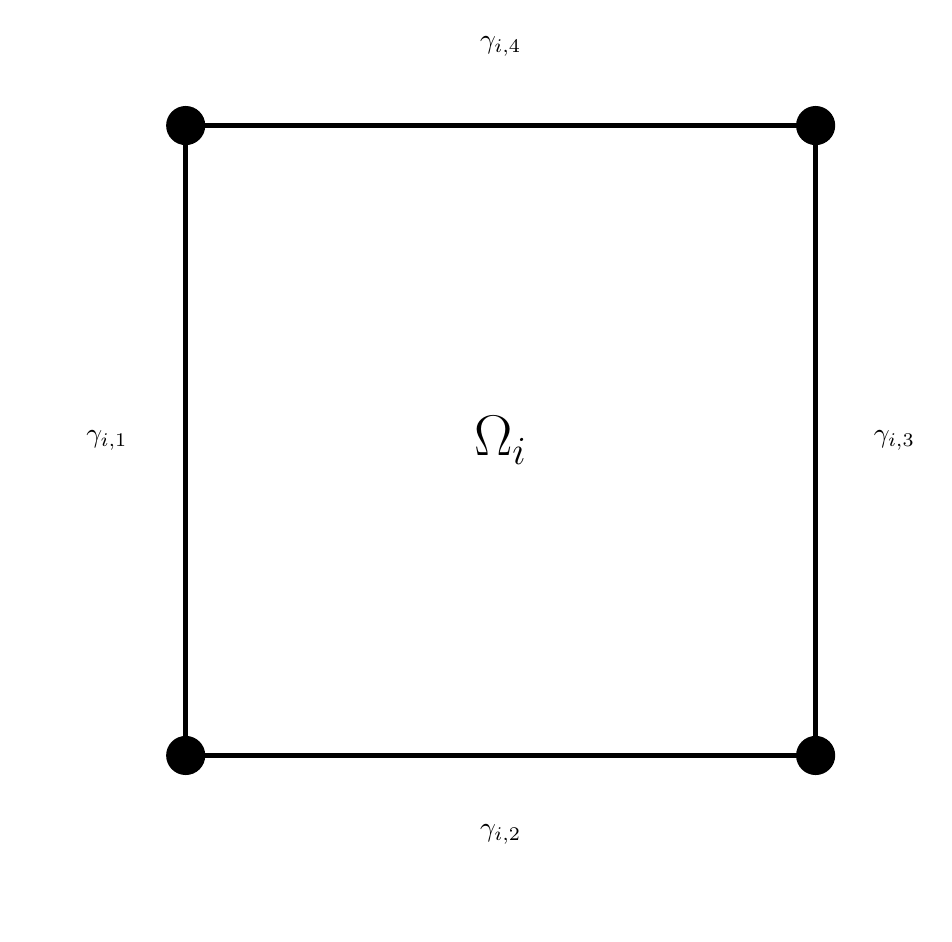
\begin{tikzpicture}[scale=2]
		\draw[line width=2pt] (1,1) rectangle (5,5);
		\draw (1,1) node[circle,fill,inner sep=5pt]{};
		\draw (1,5) node[circle,fill,inner sep=5pt]{};
		\draw (5,1) node[circle,fill,inner sep=5pt]{};
		\draw (5,5) node[circle,fill,inner sep=5pt]{};
		\node at (3,3) {\huge $\Omega_i$};
		\node at (0.5,3) {$\gamma_{i,1}$};
		\node at (3,0.5) {$\gamma_{i,2}$};
		\node at (5.5,3) {$\gamma_{i,3}$};
		\node at (3,5.5) {$\gamma_{i,4}$};
		\draw[white] (0,0) -- (5,0);
	\end{tikzpicture}
	\vspace{-3cm}
\end{wrapfigure}


\vfill\null
\columnbreak


%----------------------------------------------------------------------------------------
%	Approach
%----------------------------------------------------------------------------------------

% I'm intentionally leaving in subsections here so we can see how to do them.

\section*{Approach}


\color{MidnightBlue}
\subsection*{Transparency}
\color{Black}

% \input{filename.tex}
Lorem ipsum dolor sit amet, consectetur adipisicing elit, sed do eiusmod
tempor incididunt ut labore et dolore magna aliqua. Ut enim ad minim veniam,
quis nostrud exercitation ullamco laboris nisi ut aliquip ex ea commodo
consequat. Duis aute irure dolor in reprehenderit in voluptate velit esse
cillum dolore eu fugiat nulla pariatur. Excepteur sint occaecat cupidatat non
proident, sunt in culpa qui officia deserunt mollit anim id est laborum.

Lorem ipsum dolor sit amet, consectetur adipisicing elit, sed do eiusmod
tempor incididunt ut labore et dolore magna aliqua. Ut enim ad minim veniam,
quis nostrud exercitation ullamco laboris nisi ut aliquip ex ea commodo
consequat. Duis aute irure dolor in reprehenderit in voluptate velit esse
cillum dolore eu fugiat nulla pariatur. Excepteur sint occaecat cupidatat non
proident, sunt in culpa qui officia deserunt mollit anim id est laborum.

\color{DarkRed}
\subsection*{Small multiples}
\color{Black}

% input{filename.tex}

\begin{centering}\color{Black}
	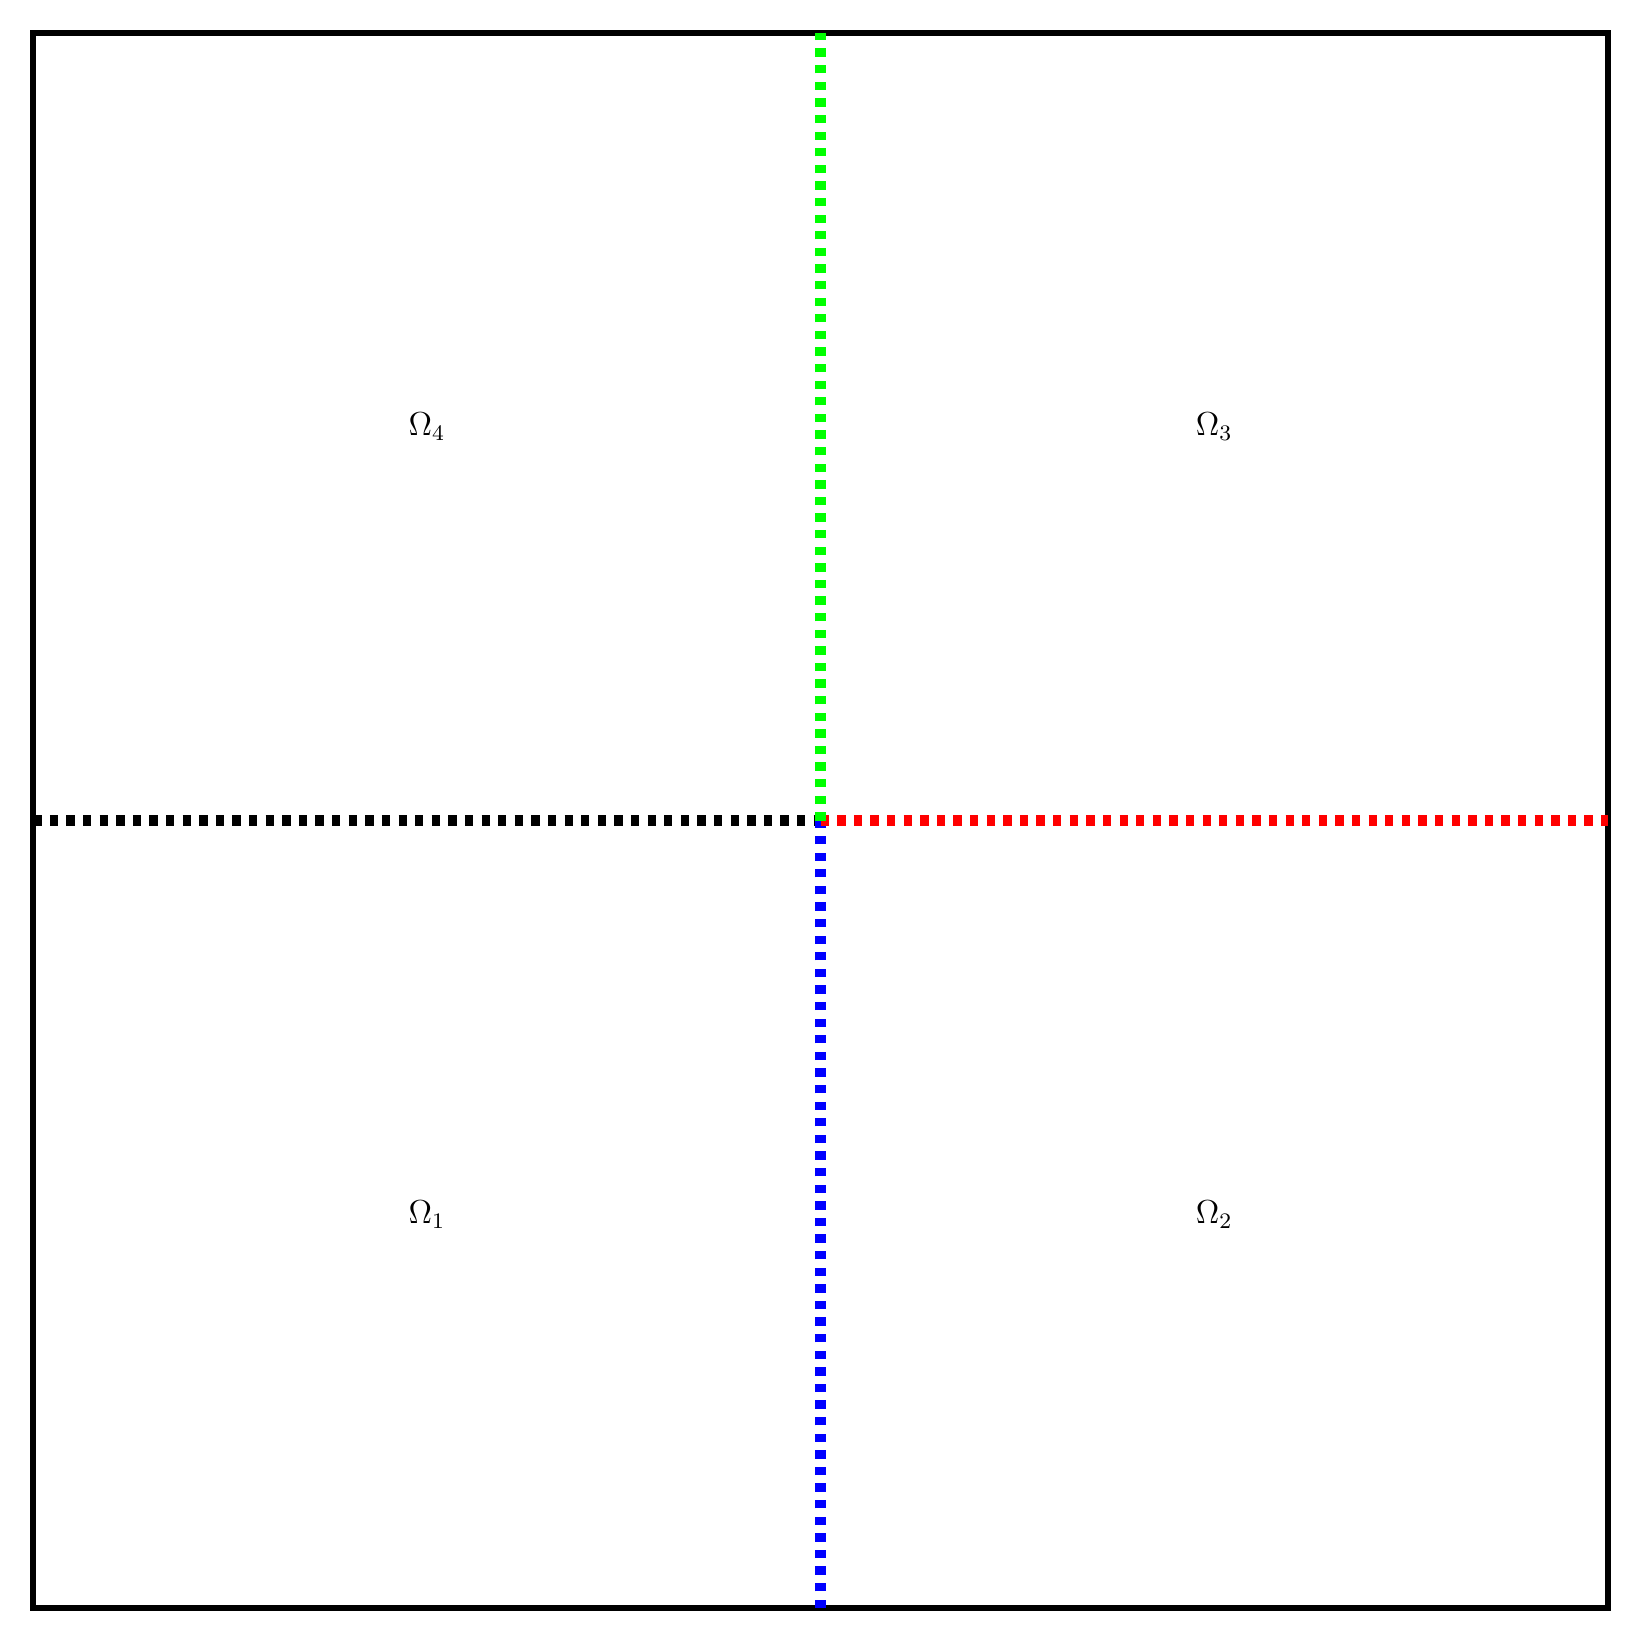
\begin{tikzpicture}[scale=5]
		\draw[step=2cm, line width=2pt](0,0) rectangle (4,4);
		\node at (1,1) {\large $\Omega_1$};
		\node at (3,1) {\large $\Omega_2$};
		\node at (1,3) {\large $\Omega_4$};
		\node at (3,3) {\large $\Omega_3$};
		\draw[black,line width=4pt,dashed] (0,2) -- (2,2);
		\draw[blue,line width=4pt,dashed] (2,0) -- (2,2);
		\draw[red,line width=4pt,dashed] (2,2) -- (4,2);
		\draw[green,line width=4pt,dashed] (2,2) -- (2,4);
	\end{tikzpicture}
	% \captionof{figure}{test caption}
\end{centering}


% \color{DarkOliveGreen}
\color{DarkGreen}
\subsection*{Moving boundaries}
% \color{DarkOliveGreen}
\color{Black}

% \input{filename.tex}


%----------------------------------------------------------------------------------------
%	Results
%----------------------------------------------------------------------------------------

\color{Black}
\section*{Results}

Screenshots and a working demo, and an indication of how they effectively address your problem.


Lorem ipsum dolor sit amet, consectetur adipisicing elit, sed do eiusmod
tempor incididunt ut labore et dolore magna aliqua. Ut enim ad minim veniam,
quis nostrud exercitation ullamco laboris nisi ut aliquip ex ea commodo
consequat. Duis aute irure dolor in reprehenderit in voluptate velit esse
cillum dolore eu fugiat nulla pariatur. Excepteur sint occaecat cupidatat non
proident, sunt in culpa qui officia deserunt mollit anim id est laborum.
Lorem ipsum dolor sit amet, consectetur adipisicing elit, sed do eiusmod
tempor incididunt ut labore et dolore magna aliqua. Ut enim ad minim veniam,
quis nostrud exercitation ullamco laboris nisi ut aliquip ex ea commodo
consequat. Duis aute irure dolor in reprehenderit in voluptate velit esse
cillum dolore eu fugiat nulla pariatur. Excepteur sint occaecat cupidatat non
proident, sunt in culpa qui officia deserunt mollit anim id est laborum.

\vspace{1cm}
\begin{centering}
	\begin{tabular}{c c c c c}
		
		{\bf h} & {\bf Offline time (s)} & {\bf FEM approximation (s)} & {\bf Our approximation (s)} & {\bf Modes per port}\\
		
		$1/36$ 	&25  	&0.12	&0.02	&25 \\
		% \hline
		$1/72$ 	&65  	&0.43	&0.03	&28 \\
		% \hline
		$1/144$	&240 	&1.86	&0.03	&31 \\
		% \hline
		$1/288$	&983	&9.26	&0.03	&32 \\
	\end{tabular}
\end{centering}


Lorem ipsum dolor sit amet, consectetur adipisicing elit, sed do eiusmod
tempor incididunt ut labore et dolore magna aliqua. Ut enim ad minim veniam,
quis nostrud exercitation ullamco laboris nisi ut aliquip ex ea commodo
consequat. Duis aute irure dolor in reprehenderit in voluptate velit esse
cillum dolore eu fugiat nulla pariatur. Excepteur sint occaecat cupidatat non
proident, sunt in culpa qui officia deserunt mollit anim id est laborum.
Lorem ipsum dolor sit amet, consectetur adipisicing elit, sed do eiusmod
tempor incididunt ut labore et dolore magna aliqua. Ut enim ad minim veniam,
quis nostrud exercitation ullamco laboris nisi ut aliquip ex ea commodo
consequat. Duis aute irure dolor in reprehenderit in voluptate velit esse
cillum dolore eu fugiat nulla pariatur. Excepteur sint occaecat cupidatat non
proident, sunt in culpa qui officia deserunt mollit anim id est laborum.

Lorem ipsum dolor sit amet, consectetur adipisicing elit, sed do eiusmod
tempor incididunt ut labore et dolore magna aliqua. Ut enim ad minim veniam,
quis nostrud exercitation ullamco laboris nisi ut aliquip ex ea commodo
consequat. Duis aute irure dolor in reprehenderit in voluptate velit esse
cillum dolore eu fugiat nulla pariatur. Excepteur sint occaecat cupidatat non
proident, sunt in culpa qui officia deserunt mollit anim id est laborum.



% \begin{center}\vspace{1cm}
% \begin{tabular}{l l l l}
% \toprule
% \textbf{Treatments} & \textbf{Response 1} & \textbf{Response 2} \\
% \midrule
% Treatment 1 & 0.0003262 & 0.562 \\
% Treatment 2 & 0.0015681 & 0.910 \\
% Treatment 3 & 0.0009271 & 0.296 \\
% \bottomrule
% \end{tabular}
% \captionof{table}{\color{Green} Table caption}
% \end{center}\vspace{1cm}

%----------------------------------------------------------------------------------------
%	CONCLUSIONS
%----------------------------------------------------------------------------------------


% \section*{Questions}
% \begin{itemize}
% 	\item Can this procedure handle nonzero right-hand side functions?
% 	\item What about non-square components?
% \end{itemize}

% \color{DarkSlateGray} % Set the color back to DarkSlateGray for the rest of the content

%----------------------------------------------------------------------------------------
%	FORTHCOMING RESEARCH
%----------------------------------------------------------------------------------------

% \color{SaddleBrown} % SaddleBrown color for the conclusions to make them stand out
\section*{Future work?}
\begin{itemize}
	\item thing 1
	\item thing 2
	\item thing 3
\end{itemize}

 %----------------------------------------------------------------------------------------
%	REFERENCES
%----------------------------------------------------------------------------------------
\color{Gray}
% \nocite{*} 	% Print all references regardless of whether they were cited in the poster or not
\nocite{bader2017static,brenner2007mathematical}
\bibliographystyle{plain} % Plain referencing style
\bibliography{bibliography} 

%----------------------------------------------------------------------------------------
%	ACKNOWLEDGEMENTS
%----------------------------------------------------------------------------------------

% \section*{Acknowledgements}
%
% Etiam fermentum, arcu ut gravida fringilla, dolor arcu laoreet justo, ut imperdiet urna arcu a arcu. Donec nec ante a dui tempus consectetur. Cras nisi turpis, dapibus sit amet mattis sed, laoreet.

%----------------------------------------------------------------------------------------

\end{multicols}
\end{document}